\chapter{Methodology}
In this chapter, each step that we followed in our method will be explained in detail.
\section{Structural Variation Discovery with HTS Data}
Structural variations are believed to be highly associated with diseases \cite{fanciulli2007fcgr3b,fellermann2006chromosome,aitman2006copy,gonzalez2005influence}. Therefore their discovery will be of critical importance in reducing the genetic disease susceptibility. Despite their significance in understanding disease susceptibility, there is no algorithm yet to find all types and sizes of structural variations at once. Before high-throughput sequencing technologies, microarrays were mainly used in structural variation discovery especially for copy number variation \cite{alkan2011genome}. As reviewed by Alkan et al., microarrays are no good at discovering balanced rearranagements and also are not able to locate the copy number variations \cite{alkan2011genome}. 

Although some are originally designed for old sequencing technologies, high-throughput sequencing platforms have brought novel methods for structural variation discovery. 
\subsection{Read Pair}
Paired-end sequencing is a sequencing method where reads are generated from both sides of a DNA fragment whose distance known. The distance information will be used later by the aligner while aligning the paired-end reads to the reference genome. Read pair method utilizes the distance information between paired-end reads \cite{tuzun2005fine}. As shown in the Figure \ref{readpair}, paired-end reads that align too distant from each other indicates a deletion, those align too close to each other indicates an insertion.

\begin{figure}[ht]
    \centering
    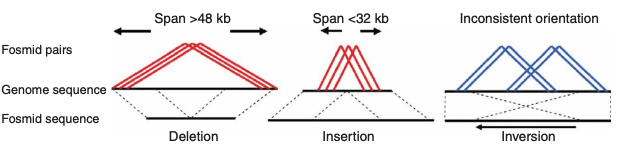
\includegraphics[scale=0.4]{images/readpair.png}
    \caption{(adapted from \cite{tuzun2005fine})}
    \label{readpair}
\end{figure}
\subsection{Read Depth}
Read depth is a simple method to detect duplications and deletions at a higher resolution. Based on the assumption that regions are randomly sequenced, for reads that are mapped to all possible locations of the reference genome, the depth of duplicated regions will be higher and the depth of deleted regions will be lower than average \cite{bailey2002recent} as shown in Figure \ref{readdepth}. Multiple read-mapping is an important aspect of read depth to work effectively. Otherwise the difference of depth between duplicated regions and deleted regions will be insignificant. However known sequencing bias against GC-rich and GC-poor regions \cite{smith2008rapid} should be handled carefully.

\begin{figure}[ht]
    \centering
    
\includegraphics[scale=0.4]{images/placeholder.jpg}
    \caption{Read depth figure will be added}
    \label{readdepth}
\end{figure}

\subsection{Split Read}
Originally designed for longer reads (Sanger sequence etc.), split read based methods were capable of structural variation discovery at one base pair resolution by trying to map the reads by splitting. Similar to read pair, the location of split reads will tell the class of structural variation. For instance, the distance between split reads shows an insertion or first split coming after second split indicates an inversion.

\subsection{Sequence Assembly}
Although it is in its early stages, sequence assembly methods are, in theory, powerful and requires less computational power. Assuming the whole genome is assembled without using the reference genome (\textit{de novo} assembly), we can easily detect structural variation by comparing the individual's genome with the reference genome.

\section{Data Preprocessing}
We have the data showing the genome-wide segmental duplications (SD). The data consist of 51,599 SD pairs with their exact locations. Furthermore, we have global alignments of SD pairs in files generated using a sequence alignment tool called ClustalW \cite{thompson1994clustal}. Since entries in our data show the duplications in pairs, we had to turn these pairs into a multiple sequence alignment in order to locate singly unique nucleotide positions. However, our data lack some pairs. For example, we have SD pairs of A-B and B-C, therefore A-C should also be in our data whereas there is not in some cases. Using the algorithm \ref{missingPairs}, we have identified 21,023 new SD pairs using existing pairs and have them aligned.

\begin{algorithm}
\caption{An algorithm to find missing SD pairs}
\label{missingPairs}
\begin{algorithmic}[1]
\Procedure{Find\_Missing\_Pairs}{}
\State $\textit{M} \gets \text{map of }\textit{Segmental Duplications}\text{ as read from data}$
\For{$\text{each key-value pair in }\textit{M}$}
\State {$\text{Let } \textit{temp\_set} \text{ be an empty set} $}
\For{$\text{values in M{[key]}}$}
\State $\textit{temp\_set} \gets \textit{temp\_set} \cup \text{M{[value]}}$
\State $\text{clear M{[value]}}$
\EndFor
\While{true}
\State $\textit{flag} \gets \text{true}$
\For{$\text{each key-value pair in }\textit{M}$}
\State $\textit{Find intersection of }\textit{temp\_set}\text{ and }\textit{value}$
\If{$\text{intersection is not empty}$}
\State $\textit{temp\_set} \gets \textit{temp\_set} \cup \text{M{[value]}}$
\State $\textit{flag} \gets \text{false}$
\EndIf
\EndFor
\If{$ \textit{flag} \text{ is true} $}
\State $\textbf{break}$
\EndIf
\EndWhile
\EndFor
\EndProcedure
\end{algorithmic}
\end{algorithm}

\section{Singly Unique Nucleotides}
Structural variation discovery has always been problematic since they tend to overlap with segmental duplications \cite{sudmant2010diversity}. Researchers that were unable to discriminate slight differences in these regions which prevents copy number variation from being accurately predicted have excluded these highly active regions from their studies. They have instead focused on unique regions of the genome.

In nearly identical regions, nucleotide difference information can be useful in discriminating segmental duplications from each other. Singly unique nucleotide (SUN) is a nucleotide difference between segmental duplications as shown red in figure \ref{singlyUniqueNucleotide}. A nucleotide difference is called a SUN if and only if they reside in only one paralog. Otherwise, as shown blue in the figure, they are called  paralogous sequence variant (PSV). 
\begin{figure}[ht]
    \centering
    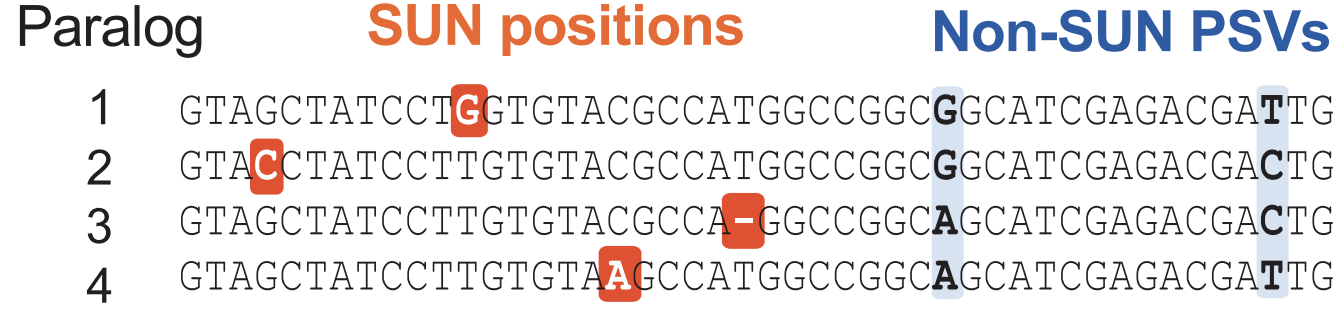
\includegraphics[scale=0.4]{images/singlyUniqueNucleotide.png}
    \caption{Singly unique nucleotide adopted from \cite{sudmant2010diversity}}
    \label{singlyUniqueNucleotide}
\end{figure}

\subsection{Extracting Singly Unique Nucleotides}
In order for paralogous sequences to be accurately identified, we need a database of positions and letters of all SUNs that reside in a segmental duplication. Instead of aligning paralogs using a multiple sequence alignment tool, which requires quite some time and computational power, it could be done using pairwise alignments of paralogs which we have in our hand (figure \ref{alignmentFile}). Let $A$, $B$ and $C$ are three paralogs and  $S_{ab}$ denotes the singly unique nucleotides of $A$ relative to $B$. The singly unique nucleotides of A will be $S_{ab} \cap S_{ac}$. The same equation is valid for other paralogs respectively. Therefore, we could figure out all SUN positions as $(S_{ab} \cap S_{ac}) \cup (S_{ba} \cap S_{bc}) \cup (S_{ca} \cap S_{cb})$.

\begin{figure}[ht]
    \centering
    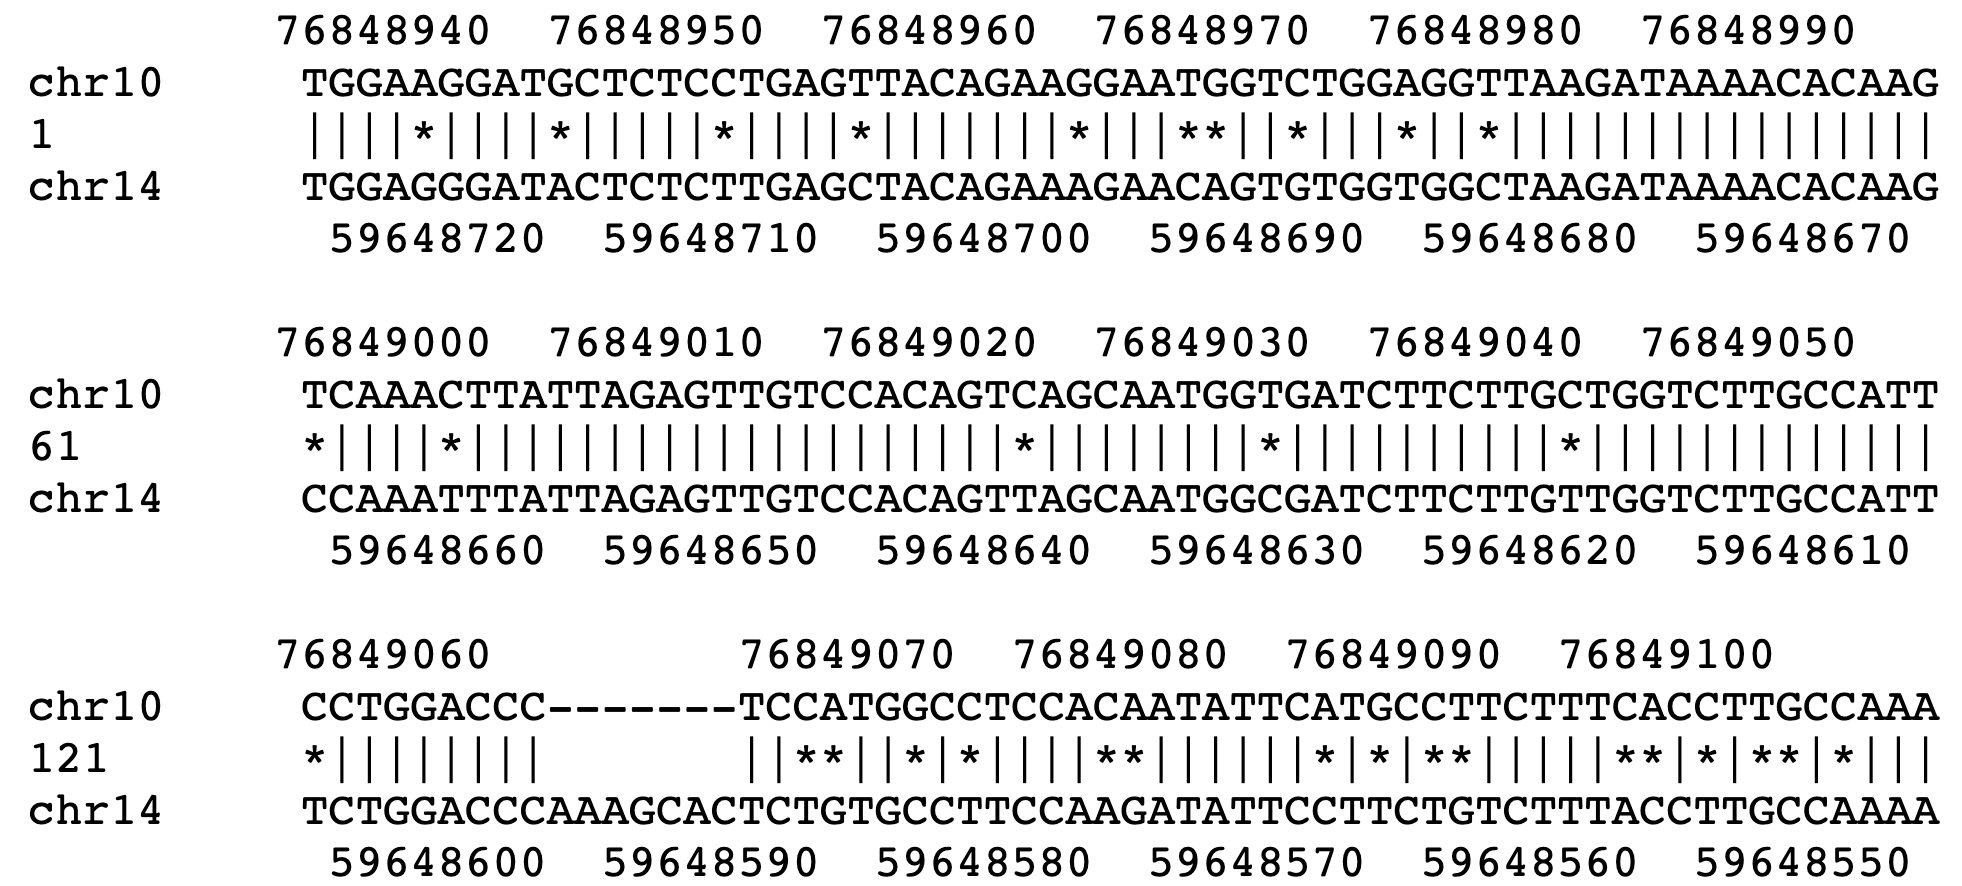
\includegraphics[scale=0.4]{images/alignmentFile.png}
    \caption{A sample screenshot from an alignment file}
    \label{alignmentFile}
\end{figure}

Algorithm \ref{getRelativeSun} uses an alignment file to find the pairwise SUN positions and letters. As shown in figure \ref{alignmentFile}, an alignment file contains the DNA sequences of two segments and an alignment results between them. The symbols $*$, $|$ and space denote a match, a mismatch and an indel respectively. It is important to state that, if there is a deletion in one sequence, every nucleotide position opposite of the deletion will be counted as a SUN. On the other hand, the deletion will be counted as one SUN. Another thing to pay attention is the strand of the sequences. Segmental duplications can be found in opposite strand of the DNA. In that case, the nucleotide in the alignment file will be replaced by its complement before getting saved to SUN database.

\begin{algorithm}
\caption{An algorithm to find pairwise SUN locations and letters}
\label{getRelativeSun}
\begin{algorithmic}[1]
\Procedure{Get\_Relative\_SUN}{alignment\_file\_path, strand}
\State $\text{Open alignment file}$
\If{file is open}
\State $\text{Let } S_{ab} \text{ and } S_{ba} \text{ empty sets}$
\While{getline(file) $\neq$ EOF}
\State{seq1 $\gets$ getline(file)}
\State{aligment $\gets$ getline(file)}
\State{seq2 $\gets$ getline(file)}
\For{$ i\gets0 \text{ to size of } \textit{alignment}$}
\If{$\textit{strand} \text{ is } -1$}
\State{seq2[i] $\gets$ \textit{GET\_OPPOSITE\_PAIR}(seq2[i]) /* It} 
\State{returns the complement of the input nucleotide, for example} 
\State{if input is A, T is returned etc.*/}
\EndIf
\If{alignment[i] is `*'}
\State{$S_{ab} \gets S_{ab} \cup seq1[i]$}
\State{$S_{ba} \gets S_{ba} \cup seq2[i]$}
\EndIf
\If{alignment[i] is ` '}
\If{seq1[i] is `-'}
\State{$S_{ba} \gets S_{ba} \cup seq2[i]$}
\EndIf
\If{seq2[i] is `-'}
\State{$S_{ab} \gets S_{ab} \cup seq1[i]$}
\EndIf
\EndIf
\EndFor
\EndWhile
\EndIf
\EndProcedure
\end{algorithmic}
\end{algorithm}


\begin{algorithm}
\caption{An algorithm to find all SUN locations and letters}
\label{allSun}
\begin{algorithmic}[1]
\Procedure{Get\_All\_SUN}{duplication\_file\_path}
\State $\text{Open duplication file}$
\If{file is open}
\State {Let singly\_unique\_nucleotide\_map an empty map showing DNA }
\State {sequence and SUN locations as key-value pair}
\For{each entry in duplication file}
\State{$\text{alignment\_file\_path} \gets \text{parsed from duplication file}$}
\State{$\text{strand} \gets \text{parsed from duplication file}$}
\State{$S_{ab}\text{, } S_{ba} \gets \textit{GET\_RELATIVE\_SUN}(\text{alignment\_file\_path, strand})$}
\EndFor
\EndIf
\EndProcedure
\end{algorithmic}
\end{algorithm}
\section{Depth of Coverage}
\subsection{GC Correction}
